\documentclass[11pt,a4paper]{article}
\usepackage[spanish,es-nodecimaldot]{babel}	% Utilizar español
\usepackage[utf8]{inputenc}					% Caracteres UTF-8
\usepackage{graphicx}						% Imagenes
\usepackage[hidelinks]{hyperref}			% Poner enlaces sin marcarlos en rojo
\usepackage{fancyhdr}						% Modificar encabezados y pies de pagina
\usepackage{float}							% Insertar figuras
\usepackage[textwidth=390pt]{geometry}		% Anchura de la pagina
\usepackage[nottoc]{tocbibind}				% Referencias (no incluir num pagina indice en Indice)
\usepackage{enumitem}						% Permitir enumerate con distintos simbolos
\usepackage[T1]{fontenc}					% Usar textsc en sections
\usepackage{amsmath, yhmath}						% Símbolos matemáticos
\usepackage{subcaption}
\usepackage{longtable}

% Comando para poner el nombre de la asignatura
\newcommand{\asignatura}{Simulación de Sistemas}
\newcommand{\autor}{Vladislav Nikolov Vasilev}
\newcommand{\titulo}{Práctica 3}
\newcommand{\subtitulo}{Modelos de Simulación Dinámicos y Discretos}

% Configuracion de encabezados y pies de pagina
\pagestyle{fancy}
\lhead{\autor{}}
\rhead{\asignatura{}}
\lfoot{Grado en Ingeniería Informática}
\cfoot{}
\rfoot{\thepage}
\renewcommand{\headrulewidth}{0.4pt}		% Linea cabeza de pagina
\renewcommand{\footrulewidth}{0.4pt}		% Linea pie de pagina

\begin{document}
\pagenumbering{gobble}

% Pagina de titulo
\begin{titlepage}

\begin{minipage}{\textwidth}

\centering


\includegraphics[scale=0.5]{img/ugr.png}\\

\textsc{\Large \asignatura{}\\[0.2cm]}
\textsc{GRADO EN INGENIERÍA INFORMÁTICA}\\[1cm]

\noindent\rule[-1ex]{\textwidth}{1pt}\\[1.5ex]
\textsc{{\Huge \titulo\\[0.5ex]}}
\textsc{{\Large \subtitulo\\}}
\noindent\rule[-1ex]{\textwidth}{2pt}\\[3.5ex]

\end{minipage}

\vspace{0.5cm}

\begin{minipage}{\textwidth}

\centering

\textbf{Autor}\\ {\autor{}}\\[2.5ex]
\textbf{Rama}\\ {Computación y Sistemas Inteligentes}\\[2.5ex]
\vspace{0.3cm}


\includegraphics[scale=0.3]{img/etsiit.jpeg}

\vspace{0.7cm}
\textsc{Escuela Técnica Superior de Ingenierías Informática y de Telecomunicación}\\
\vspace{1cm}
\textsc{Curso 2019-2020}
\end{minipage}
\end{titlepage}

\pagenumbering{arabic}
\tableofcontents
\thispagestyle{empty}				% No usar estilo en la pagina de indice

\newpage

\setlength{\parskip}{1em}

\section{\textsc{Mi segundo modelo de simulación discreto}}

En esta sección vamos a estudiar primero el comportamiento de un modelo de
simulación de un servidor con una única cola, y después de $m$ servidores
con una única cola. Vamos a ver cómo distintos métodos de incremento del
itempo pueden afectar al funcionamiento del sistema, y discutiremos cuál
de ellos es mejor.

\subsection{Método de incremento fijo del tiempo}

El primer método de incremento del tiempo que vamos a estudiar es el incremento
fijo. Como su propio nombre indica, el tiempo se va incrementando en una cantidad
fija, tal como lo hace un reloj normal. Esta cantidad viene decidida por la persona
que va a utilizar el sistema (pueden ser minutos, segundos, milésimas, horas, etc.).

Debido a la naturaleza de dicho incremento, la variable de tiempo debe ser tratada
como una variable entera. Por tanto, aunque en el pesudocódigo proporcionado se
generen las llegadas y el servicio utilizando valores reales, dichos valores obtenidos
deben ser transformados a enteros, redondeándolos al entero más próximo. Además, si
el valor que se obtiene al hacer las transformaciones correspondientes es 0, se
debe devolver 1, ya que si no, se generaría un suceso en el tiempo actual y, al
incrementar el tiempo en una unidad, ese suceso se quedaría en un tiempo anterior
al nuevo actual, y por tanto, nunca se podría llevar a cabo.

Una vez dicho esto, vamos a experimentar con el sistema. Para ello, vamos a utilizar
las siguientes unidades de tiempo: horas, medias horas, cuartos de hora, minutos, segundos,
décimas de segundo y milésimas de segundo. En cada caso simularemos que se tienen que
atender 10000 clientes, y repetiremos cada ejecución 100 veces. De ahí, podremos
ver los valores obtenidos en cada simulación y los valores medios para el número
medio de clientes en la cola y el porcentaje de tiempo de ocio del servidor. Además,
veremos cuánto tarda cada simulación y el tiempo medio que han tardado todas las simulaciones,
aunque en la tabla se reflejará solo este último valor. Vamos a pintar también en algunos de los
casos gráficas para ver cómo van evolucionando los resultados que se obtienen en cada una de las
100 simulaciones, para ver si de verdad se parecen a los resuldatos medios. Los valores de
\texttt{tlleg} y \texttt{tserv} son 9 y 6 minutos, respectivamente, aunque aparecerán reflejados
según la unidad de tiempo correspondiente.

Una vez hechas todas las simulaciones, se han obtenido los siguientes resultados:

\begin{table}[H]
\resizebox{\textwidth}{!}{%
\begin{tabular}{|c|c|c|c|c|}
\hline
\texttt{tlleg} & \texttt{tserv} & \textbf{\begin{tabular}[c]{@{}c@{}}Num. medio\\ clientes cola\end{tabular}} & \textbf{\begin{tabular}[c]{@{}c@{}}\% medio tiempo\\ ocio servidor\end{tabular}} & \textbf{\begin{tabular}[c]{@{}c@{}}Tiempo ejecución\\ medio\end{tabular}} \\ \hline
0.15 & 0.1 & 0.0262607 & 0.138175 & 0.000593755 \\ \hline
0.3 & 0.2 & 0.21363 & 2.93386 & 0.000889945 \\ \hline
0.6 & 0.4 & 0.550758 & 11.669 & 0.000932894 \\ \hline
9 & 6 & 1.25962 & 31.5821 & 0.00104538 \\ \hline
540 & 360 & 1.33738 & 33.3778 & 0.0119809 \\ \hline
5400 & 3600 & 1.32336 & 33.4474 & 0.134477 \\ \hline
54000 & 36000 & 1.344 & 33.1509 & 1.33758 \\ \hline
\end{tabular}%
}
\caption{Resultados obtenidos por el incremento de tiempo fijo.}
\label{tab:fijo}
\end{table}

A primera vista podemos ver que a medida que \texttt{tlleg} y \texttt{tserv}
usan unidades más pequeñas de tiempo (y por tanto, sus valores son más altos),
los resultados obtenidos se van incrementando, hasta el punto en el que parece
que se estabilizan. Lo que sucede es que cuando las unidades de tiempo son grandes,
los valores de \texttt{tlleg} y \texttt{tserv} son menores que 0. Al llamar a
los generadores, se producirán valores próximos a 0, y al redondearlos, estos pasan
a valer 0. Como el generador no puede devolver 0, devuelve 1. Por tanto, lo que
estamos haciendo en realidad es sobreestimar la duración de un suceso, por lo que
los valores obtenidos no serán reales, ya que se va acumulando el error al haber
sobreestimado. Este es un problema de los métodos de incremento fijo del tiempo, y
a la vez es una fuerte desventaja, ya que dependiendo de la unidad de tiempo que se
utilice, los valores obtenidos serán más o menos representativos de los que se podrían
obtener de forma teórica.

Aparte de esto, si analizamos los resultados vemos que los tiempos medios de ejecución
se van incrementando, debido a que se debe incrementar más veces el reloj hasta
llegar a un suceso. El valor medio del número medio de clientes en cola, $Q(n)$, parece
estabilizarse en torno a 1.33, y el valor medio del porcentaje de tiempo de ocio
del servidor, $PTO(n)$ parece estabilizarse al final en torno al 33\%. Para unidades
de tiempo superiores a los segundos los resultados obtenidos no son representativos,
ya que se quedan demasiado lejos de los valores obtenidos al utilizar unidades
de tiempo más pequeñas. Por tanto, parece ser que, en caso de utilizar generadores
de incremento fijo, lo suyo sería utilizar unidades de tiempo más pequeñas (es decir,
que los valores sean grandes), ya que de esta forma se cometerá menos error.

Ahora, pasemos a estudiar el comportamiento del sistema para cada simulación.
Vamos a ver qué resultados se han obtenido para el número de medio de clientes
en cola y para el porcentaje de tiempo de ocio del servidor. Vamos a estudiar
dicha evolución con gráficas, tal y como se mencionó anteriormente, para ver
si hay mucha discrepancia entre los valores medios obtenidos. Vamos a realizar
un estudio de todos los resultados de forma conjunta.

A continuación se pueden ver las gráficas mencionadas en el párrafo anterior:

\begin{figure}[H]
	\centering
	\begin{subfigure}{.5\textwidth}
		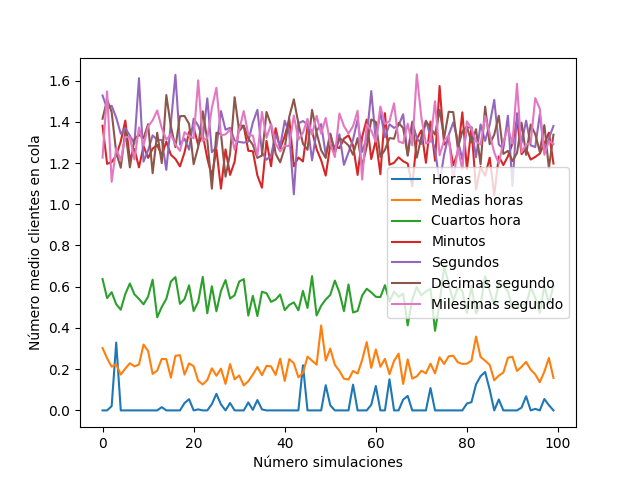
\includegraphics[scale=0.44]{img/fijo-q}
		\subcaption{Número medio de clientes en la cola.}
		\label{fig:fijo-q}
	\end{subfigure}%
	~
	\begin{subfigure}{.5\textwidth}
		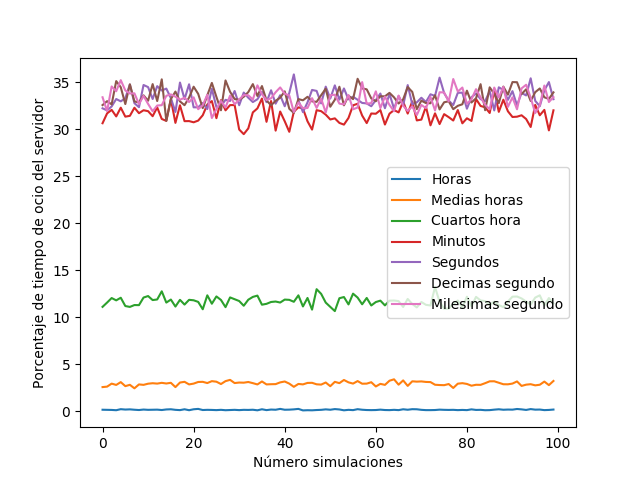
\includegraphics[scale=0.44]{img/fijo-pto}
		\subcaption{Porcentaje de tiempo de ocio del servidor.}
		\label{fig:fijo-pto}
	\end{subfigure}

	\caption{Variación de los resultados a lo largo de las simulaciones.}
	\label{fig:fijo}
\end{figure}

Vemos que, tal y como habíamos dicho antes, para unidades de tiempo más grandes
que los minutos, los valores de $Q(n)$ y $PTO(n)$ están bastante alejados del resto.
En aquellos casos en los que se usa como unidad de tiempo una que es el minuto
o inferior a ésta los resultados sí que están próximos, y parece que se aproximan
a los valores medios obtenidos. Vemos que en todos los casos existe cierta variabilidad
entre los resultados de una simulación o de otra. Por tanto, no podríamos fiarnos solo
de los resultados obtenidos por una simulación, sino que, tal y como llevamos haciendo
hasta ahora, habría que hacer algunas simulaciones y promediar.

Por tanto, como pequeña conclusión de esta parte, podemos sacar que es importante
escoger una unidad de tiempo adecuada, ya que si no lo es, va a provocar que
los resultados no sean del todo buenos. Si hemos escogido una unidad de
tiempo adecuada, los resultados que obtengamos serán buenos, ya que estarán bastante
relacionados entre sí, justo como ha pasado aquí.

\subsection{Método de incremento variable del tiempo}

El siguiente método de incremento del tiempo que vamos a estudiar es el incremento
variable. En este caso, el tiempo no se va incrementando de manera fija como sucedía
anteriormente, si no que se incrementa hasta el suceso más próximo de una. Por
tanto, este método parece ser mucho más eficiente, ya que evita tener que pegar demasiados
saltos y evita errores como los que se producían anteriormente.

Para ver como funciona este tipo de incremento, vamos a realizar los mismos experimentos
que en la sección anterior, de forma que tengamos resultados comparables. A continuación
se puede ver una tabla con los resultados:

\begin{table}[H]
\resizebox{\textwidth}{!}{%
\begin{tabular}{|c|c|c|c|c|}
\hline
\texttt{tlleg} & \texttt{tserv} & \textbf{\begin{tabular}[c]{@{}c@{}}Num. medio\\ clientes cola\end{tabular}} & \textbf{\begin{tabular}[c]{@{}c@{}}\% medio tiempo\\ ocio servidor\end{tabular}} & \textbf{\begin{tabular}[c]{@{}c@{}}Tiempo ejecución\\ medio\end{tabular}} \\ \hline
0.15 & 0.1 & 1.32894 & 33.3767 & 0.000731009 \\ \hline
0.3 & 0.2 & 1.32033 & 33.4927 & 0.000986358 \\ \hline
0.6 & 0.4 & 1.335 & 33.3979 & 0.000692968 \\ \hline
9 & 6 & 1.32356 & 33.5117 & 0.000969834 \\ \hline
540 & 360 & 1.35058 & 33.1523 & 0.000713056 \\ \hline
5400 & 3600 & 1.33727 & 33.3192 & 0.000690027 \\ \hline
54000 & 36000 & 1.34364 & 33.2906 & 0.000895026 \\ \hline
\end{tabular}%
}
\caption{Resultados obtenidos por el incremento de tiempo variable.}
\label{tab:var}
\end{table}

Podemos ver que en general los resultados obtenidos en todos los casos son más
o menos iguales, tanto para los valores de $Q(n)$ como de $PTO(n)$. Además, los
tiempos de ejecución son casi los mismos en todos los casos, por lo tanto son
independiendes de la unidad de tiempo utilizada, a diferencia del caso anterior.
Aquí los tiempos son casi constantes, ya que existe poca o muy poca variación entre
éstos. Observando los tiempos de la tabla \ref{tab:fijo}, vemos que, a medida
que usamos medidas de tiempo más pequeñas, los tiempos medios se van haciendo más grandes,
experimentando lo que parece ser un crecimiento lineal, ya que el número de veces
que se incrementará el reloj aumenta. Aquí, los incrementos solo dependen del
número de sucesos, mientras que en el caso anterior dependían de la unidad de
medida de tiempo. Por tanto, de aquí podemos concluir que, efectivamente, el
incremento variable del tiempo es muchísimo más eficiente que el incremento
fijo del tiempo, ya que el primero es constante, independientemente de la unidad
de medida utilizada, mientras que el segundo es lineal, ya que en función de la unidad
de medida del tiempo utilizada tardará más o menos (será más rápido para las unidades
más grandes).

Si comparamos la calidad de los resultados, vemos también que en general son mucho
mejores. Vemos que incluso utilizando unidades de tiempo grandes, como por ejemplo
horas, los valores medios obtenidos son muy parecidos a los que se obtienen
con unidades más pequeñas, como por ejemplo las décimas de segundo. Esto es
completamente lo opuesto a lo que sucedió anteriormente, ya que los resultados
eran muy dispares. Por tanto, parece que el incremento de tiempo variable
es independiente de la unidad de medida usada, a diferencia del incremento
fijo del tiempo.

Si observamos los resultados obtenidos en cada una de las simulaciones, nos
encontramos con lo siguiente:

\begin{figure}[H]
	\centering
	\begin{subfigure}{.5\textwidth}
		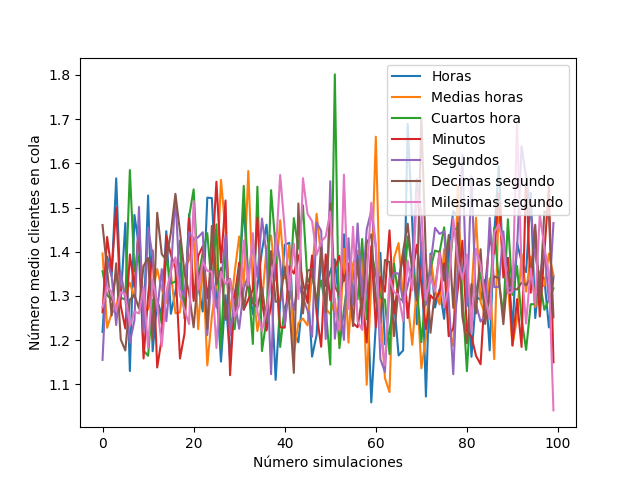
\includegraphics[scale=0.44]{img/var-q}
		\subcaption{Número medio de clientes en la cola.}
		\label{fig:var-q}
	\end{subfigure}%
	~
	\begin{subfigure}{.5\textwidth}
		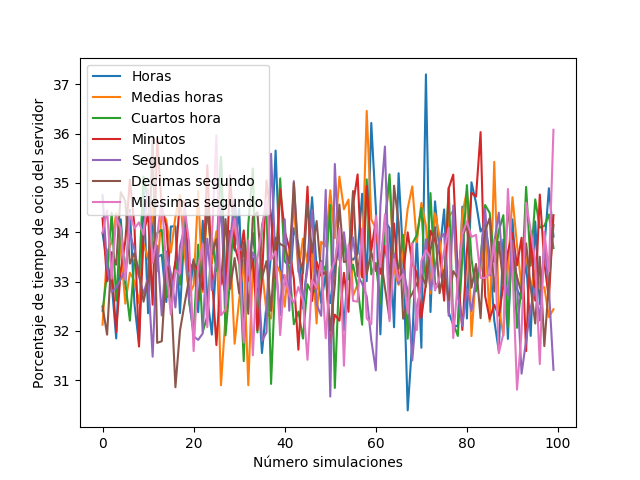
\includegraphics[scale=0.44]{img/var-pto}
		\subcaption{Porcentaje de tiempo de ocio del servidor.}
		\label{fig:var-pto}
	\end{subfigure}

	\caption{Variación de los resultados a lo largo de las simulaciones.}
	\label{fig:var}
\end{figure}

Tal y como pasaba antes, vemos que existen variaciones entre los resultados
obtenidos para cada simulación. No obstante, vemos que son bastante
parecidos en general. Parece que oscilan en torno a la media, tal y
como pasaba antes. De nuevo, si hubiésemos tomado el resultado de una única
simulación como el correcto, nos hubiésemos equivocado ya que, tal y como
hemos visto, existe una ligera variación en los resultados.

Ahora que hemos visto los dos modelos, podemos hacer una comparación de
cómo de buenos son los resultados ofrecidos. Para ello, nos podemos
servir de las expresiones teóricas. Para hacer los cálculos, vamos a utilizar
los tiempos expresados en minutos, para facilitar el cómputo. Primero
tenemos que calcular $\rho$:

\begin{equation}
	\rho = \frac{\texttt{tserv}}{\texttt{tlleg}} = \frac{6}{9} =
	\frac{2}{3} = 0.\wideparen{6}
\end{equation}

Ahora, podemos calcular el valor teórico de $Q(n)$:

\begin{equation}
	Q(n) = \frac{\rho^2}{1-\rho} = \frac{\big(\frac{2}{3}\big)^2}{1 - \frac{2}{3}} =
	\frac{\frac{4}{9}}{\frac{1}{3}} = \frac{12}{9} = \frac{4}{3} = 1.\wideparen{3}
\end{equation}

Y también el de $PTO(n)$:

\begin{equation}
	PTO(n) = 100 \cdot (1 - \rho) = 100 \cdot \Big(1 - \frac{2}{3}\Big) 
	100 \cdot \frac{1}{3} = \frac{100}{3} = 33.\wideparen{3}
\end{equation}

Si comparamos los resultados de la tabla \ref{tab:fijo} con los teóricos,
vemos que el incremento fijo de tiempo solo ofrece resultados parecidos
a los teóricos cuando las unidades de tiempo utilizadas son pequeñas.
A partir de los segundos podríamos decir realmente que son resultados correctos.
A excepción de los minutos, que ofrecen unos resultados aproximados aunque
con cierto error, las medidas de tiempo más grandes nos ofrecerían valores
con demasiado error como para considerarlos válidos.

En cambio, todos los resultados medios obtenidos por el incremento variable
del tiempo, tal y como se pueden ver en la tabla \ref{tab:var}, son muy próximos,
por no decir casi iguales, a los resultados teóricos, independientemente de
la unidad de medida del tiempo utilizada. Por tanto, la calidad de los resultados
ofrece el incremento variable del tiempo es muy superior a la del incremento fijo
del tiempo.

Como conclusión, podemos decir que, tras estudiar los dos casos, hemos visto
que el incremento variable del tiempo es órdenes de magnitud más eficiente
que el incremento fijo del tiempo, y además, permite obtener unos resultados
de mayor calidad, independientemente de qué medida del tiempo se use.

\subsection{Modelo dinámico discreto de $m$ servidores con una única cola}

En esta sección vamos a estudiar un modelo algo más complejo que el anterior,
en el cuál tenemos $m$ servidores con una única cola. Vamos a empezar a estudiar
el sistema primero con $m=1$, de forma que podamos verificar utilizando valores
teóricos. Posteriormente, estudiaremos el sistema al aumentar $m$ y haciendo
que el tiempo de servicio de los servidores se mantenga constante; es decir,
vamos a hacer que \texttt{tserv} dividido $m$ sea igual tanto para $m=1$ como
para valores más elevados. También probaremos a simular más de una vez, y además,
cambiaremos los simuladores de datos, para ver qué efecto tiene dicho cambio
sobre el sistema.

\subsubsection{Verificación del sistema}

Vamos a empezar experimentando con el servidor para ver si los resultados
ofrecidos son buenos o no. Para ello, vamos a establecer una serie de condiciones:

\begin{itemize}[label=\textbullet]
	\item Como medida del tiempo utilizaremos los minutos, ya que no se especifica
	ninguna medida concreta con la que realizar las pruebas y porque el cáclulo de los
	valores teóricos será más sencillo. Por tanto, tendremos que $\texttt{tlleg} = 9$
	y $\texttt{tserv} = 6$.
	\item Como al sistema se le tiene que especificar cuál es el tiempo de parada,
	vamos a utilizar los siguientes tiempos: 100, 1000, 10000, 100000, 1000000. De
	esta forma, vamos a ver cómo evolucionan los resultados obtenidos al hacer la
	simulación más larga.
\end{itemize}

Una vez hechas las simulaciones correspondientes, se pueden ver los resultados
a continuación:

\begin{table}[H]
\resizebox{\textwidth}{!}{%
\begin{tabular}{c|c|c|c|c|c|}
\cline{2-6}
\multicolumn{1}{l|}{} & \multicolumn{5}{c|}{\textbf{Tiempo parada}} \\ \cline{2-6} 
\textbf{} & \textbf{100} & \textbf{1000} & \textbf{10000} & \textbf{100000} & \textbf{1000000} \\ \hline
\multicolumn{1}{|c|}{\textbf{\begin{tabular}[c]{@{}c@{}}T. medio\\ espera en cola\end{tabular}}} & 14.319 & 6.660 & 9.228 & 11.988 & 11.970 \\ \hline
\multicolumn{1}{|c|}{\textbf{\begin{tabular}[c]{@{}c@{}}T. medio estancia\\ en sistema\end{tabular}}} & 20.319 & 12.660 & 15.228 & 17.988 & 17.970 \\ \hline
\multicolumn{1}{|c|}{\textbf{\begin{tabular}[c]{@{}c@{}}Núm. medio\\ clientes en cola\end{tabular}}} & 2.233 & 0.770 & 1.022 & 1.332 & 1.328 \\ \hline
\multicolumn{1}{|c|}{\textbf{\begin{tabular}[c]{@{}c@{}}Núm. medio\\ clientes en sistema\end{tabular}}} & 3.128 & 1.355 & 1.682 & 1.998 & 1.992 \\ \hline
\multicolumn{1}{|c|}{\textbf{\begin{tabular}[c]{@{}c@{}}Long. media\\ colas no vacías\end{tabular}}} & 2.860 & 2.166 & 2.474 & 3.006 & 2.996 \\ \hline
\multicolumn{1}{|c|}{\textbf{\begin{tabular}[c]{@{}c@{}}\% tiempo\\ ocio servidor\end{tabular}}} & 10.530 & 41.511 & 34.085 & 33.362 & 33.507 \\ \hline
\multicolumn{1}{|c|}{\textbf{Long. máx. cola}} & 5 & 7 & 10 & 17 & 26 \\ \hline
\end{tabular}%
}
\caption{Resultados experimentando con el tiempo de parada.}
\label{tab:colas-1}
\end{table}

Para comparar dichos resltados, vamos a calcular los valores teóricos, los
cuáles tienen sentido cuando el sistema está en funcionamiento un tiempo lo
suficientemente grande como para aproximarse a infinito. Los resultados
podemos verlos a continuación:

\begin{itemize}[label=\textbullet]
	\item Tiempo medio de espera en cola
	$= \frac{tserv^2}{tlleg-tserv} = \frac{6^2}{9-6} = \frac{36}{3} = 12$
	\item Tiempo medio de estancia en el sistema
	$= \frac{tserv \cdot tlleg}{tlleg-tserv} = \frac{6 \cdot 9}{9-6} = \frac{54}{3} = 18$
	\item Número medio de clientes en cola
	$= \frac{tserv^2}{tlleg (tlleg-tserv)} = \frac{6^2}{9\cdot (9-6)} = \frac{36}{27} = 1.\wideparen{3}$
	\item Número medio de clientes en el sistema
	$= \frac{tserv}{tlleg-tserv} = \frac{6}{9-6} = \frac{6}{3} = 2$
	\item Longitud media de colas no vacías
	$= \frac{tlleg}{tlleg-tserv} = \frac{9}{9-6} = \frac{9}{3} = 3$
	\item Porcentaje de tiempo de ocio del servidor
	$= \big(1 - \frac{tserv}{tlleg}\big) \cdot 100 = \big(1 - \frac{6}{9}\big) \cdot 100 = \frac{100}{3} = 33.\wideparen{3}$
\end{itemize}

Ahora, pasemos a analizar los resultados obtenidos. Vemos que para un tiempo de
simulación pequeño, los resultados obtenidos se alejan bastante de los teóricos,
ya que éstos últimos son para cantidades de tiempo que tienden a infinito. Notamos,
no obstante, que a medida que se aumenta el tiempo de simulación, los valores sí
que empiezan a tender a los teóricos. A partir de un tiempo de simulación de 100000
unidades vemos que los resultados ya sí que casi iguales a los teóricos, con un cierto margen
de error, obviamente. Por tanto, si quisiéramos obtener unos resultados acordes
a los teóricos para cualesquiera valores de \texttt{tlleg} y \texttt{tserv}, deberíamos
simular durante un tiempo lo suficientemente grande, siempre acorde al tamaño
de las unidades de tiempo.

\subsubsection{Aumento del número de servidores}

Vamos a aumentar ahora el número de servidores que usamos, pero vamos a aumentar
el valor de \texttt{tserv} de forma proporcional al número de servidores, tal
y como se comentó anteriormente.

Para hacer la experimentación, vamos a probar con 2, 3, 4, 5 y 10 servidores,
y por tanto, con unos valores de \texttt{tserv} de 12, 18, 24, 30 y 60.
En cada caso simularemos durante 100000 unidades de tiempo, ya que antes ha permitido
obtener unos resultados que se aproximaban a los teóricos.

\begin{table}[H]
\begin{tabular}{c|c|c|c|c|c|c|}
\cline{2-7}
\multicolumn{1}{l|}{} & \multicolumn{6}{c|}{\textbf{Número de servidores}} \\ \cline{2-7} 
\textbf{} & \textbf{1} & \textbf{2} & \textbf{3} & \textbf{4} & \textbf{5} & \textbf{10} \\ \hline
\multicolumn{1}{|c|}{\textbf{\begin{tabular}[c]{@{}c@{}}T. medio\\ espera en cola\end{tabular}}} & 11.988 & 9.288 & 7.639 & 6.999 & 5.074 & 2.548 \\ \hline
\multicolumn{1}{|c|}{\textbf{\begin{tabular}[c]{@{}c@{}}T. medio estancia\\ en sistema\end{tabular}}} & 17.988 & 21.288 & 25.639 & 30.999 & 35.074 & 62.548 \\ \hline
\multicolumn{1}{|c|}{\textbf{\begin{tabular}[c]{@{}c@{}}Núm. medio\\ clientes en cola\end{tabular}}} & 1.332 & 1.016 & 0.851 & 0.780 & 0.554 & 0.284 \\ \hline
\multicolumn{1}{|c|}{\textbf{\begin{tabular}[c]{@{}c@{}}Núm. medio\\ clientes en sistema\end{tabular}}} & 1.998 & 2.317 & 2.854 & 3.450 & 3.819 & 6.914 \\ \hline
\multicolumn{1}{|c|}{\textbf{\begin{tabular}[c]{@{}c@{}}Long. media\\ colas no vacías\end{tabular}}} & 3.006 & 3.009 & 2.846 & 3.026 & 2.798 & 2.854 \\ \hline
\multicolumn{1}{|c|}{\textbf{\begin{tabular}[c]{@{}c@{}}\% tiempo\\ ocio servidor\end{tabular}}} & 33.362 & 34.981 & 33.258 & 33.255 & 34.702 & 33.709 \\ \hline
\multicolumn{1}{|c|}{\textbf{Long. máx. cola}} & 17 & 21 & 15 & 19 & 16 & 12 \\ \hline
\end{tabular}
\caption{Resultados variando el número de servidores.}
\label{tab:colas-2}
\end{table}

Los resultados pueden verse en la tabla \ref{tab:colas-2}. Vemos que, en general,
existen mejoras al aumentar el número de servidores. Vemos que los tiempos de espera
en cola se reducen, al igual que el número medio de clientes en cola y la longitud media
de las colas no vacías. Por otro lado, el tiempo de estancia en el sistema aumenta, al
igual que el número medio de clientes en el sistema. No obstante, como podemos ver,
la longitud máxima de la cola no experimenta mucha mejora (se podrían llevar a cabo
tests estadísticos para ver si existe o no mejora significativa), y el porcentaje
de tiempo de ocio del servidor se mantiene casi constante.

Por tanto, aumentar el número de servidores del que se dispone perimite obtener en
general mejores resultados. No obstante, el tiempo de ocio va a ser el mismo en todos
los casos, con lo cuál habrá potencia de cómputo desaprovechada siempre. Por tanto,
si quisiéramos recomendar la mejor opción, tendríamos que encontrar un equilibrio entre
los resultados que queramos conseguir y el presupuesto del que dispongamos, ya que este
último factor influirá mucho a la hora de decantarnos por una u otra opcion.

\subsubsection{Cálculo de valores medios}

Lo siguiente que tenemos que hacer es modificar el sistema para que sea capaz
de realizar más de una simulación. Para ello, hace falta llevar una cuenta de
los valores que se van obteniendo, con el objetivo de poder sacar un valor medio
final a partir de ellos, junto con su correspondiente desviación típica.

Después de realizar algunas modificaciones del sistema, vamos a ver qué resultados
ofrece. Para ello, vamos a obtener una tabla parecida a las anteriores, en las que
probaremos a simular 100 y 1000 veces para distintos tiempos de parada, como por
ejemplo 1000 y 10000, para ver qué resultados medios se obtienen (si son mejores
que los que había antes) junto con su desviación típica. Los tiempos son los mismos
de antes, con lo cuál no los comentaremos.

Los resultados se pueden ver en la tabla \ref{tab:colas-repeat}. Podemos ver que al repetir las simulaciones
una serie de veces, se consiguen mejores resultados de media. Para el caso
del tiempo de parada de 1000, los resultados son peores que los de 10000. Además,
la desviación típica es bastante grande, con lo cuál existe mucha variación de los
resultados. Sin embargo, para el caso de 10000 unidades de tiempo, los resultados
son bastante buenos, sobre todo si los comparamos con los de la tabla \ref{tab:colas-1}.
En este caso se acercan más a la media, y tienen una desviación típica moderada, sin ser
tan grande como en el caso de las 1000 unidades. Por tanto, de aquí podemos concluir
que es importante realizar no una, si no un conjunto de simulaciones, y promediar
los resultados obtenidos. Este acercamiento permite obtener resultados mucho
más precisos que si simplemente se ejecuta una vez el sistema, ya que los procesos estocásticos
son mucho más notables en una única simulación que en el promedio de un conjunto de
simulaciones.

\begin{table}[H]
\centering
\resizebox{\textwidth}{!}{%
\begin{tabular}{c|c|c|c|c|}
\cline{2-5}
\textbf{} & \multicolumn{4}{c|}{\textbf{Tiempo parada}} \\ \cline{2-5} 
\multicolumn{1}{l|}{} & \multicolumn{2}{c|}{\textbf{1000}} & \multicolumn{2}{c|}{\textbf{10000}} \\ \cline{2-5} 
\textbf{} & \multicolumn{2}{c|}{\textbf{Núm. simul.}} & \multicolumn{2}{c|}{\textbf{Núm. simul.}} \\ \cline{2-5} 
\multicolumn{1}{l|}{} & \textbf{100} & \textbf{1000} & \textbf{100} & \textbf{1000} \\ \hline
\multicolumn{1}{|c|}{\textbf{\begin{tabular}[c]{@{}c@{}}T. medio\\ espera en cola\end{tabular}}} & $10.012 \pm 5.093$ & $10.690 \pm 6.705$ & $11.646 \pm 2.230$ & $11.876 \pm 2.496$ \\ \hline
\multicolumn{1}{|c|}{\textbf{\begin{tabular}[c]{@{}c@{}}T. medio estancia\\ en sistema\end{tabular}}} & $ 16.012\pm 5.093$ & $16.690 \pm 6.705$ & $17.646 \pm 2.230$ & $17.876 \pm 2.496$ \\ \hline
\multicolumn{1}{|c|}{\textbf{\begin{tabular}[c]{@{}c@{}}Núm. medio\\ clientes en cola\end{tabular}}} & $1.148 \pm 0.645$ & $1.229 \pm 0.865$ & $1.291 \pm 0.258$ & $1.326 \pm 0.298$ \\ \hline
\multicolumn{1}{|c|}{\textbf{\begin{tabular}[c]{@{}c@{}}Núm. medio\\ clientes en sistema\end{tabular}}} & $1.800 \pm 0.710$ & $1.883 \pm 0.928$ & $1.954 \pm 0.276$ & $1.992 \pm 0.319$ \\ \hline
\multicolumn{1}{|c|}{\textbf{\begin{tabular}[c]{@{}c@{}}Long. media\\ colas no vacías\end{tabular}}} & $2.557 \pm 0.849$ & $2.684 \pm 1.104$ & $2.905 \pm 0.409$ & $2.963 \pm 0.471$ \\ \hline
\multicolumn{1}{|c|}{\textbf{\begin{tabular}[c]{@{}c@{}}\% tiempo\\ ocio servidor\end{tabular}}} & $34.823 \pm 8.434$ & $34.586 \pm 8.560$ & $33.677 \pm 2.499$ & $33.371 \pm 2.803$ \\ \hline
\multicolumn{1}{|c|}{\textbf{Long. máx. cola}} & $7.230 \pm 2.730$ & $7.463 \pm 2.925$ & $12.590 \pm 2.656$ & $12.872 \pm 3.234$ \\ \hline
\end{tabular}%
}
\caption{Resultados experimentando con el número de simulaciones.}
\label{tab:colas-repeat}
\end{table}

\subsubsection{Modificando los generadores de datos}

Por úlitmo, vamos a experimentar modificando los generadores de datos para ver
cómo influyen éstos en los resultados obtenidos. Se pide implementar un generador
determinísitico, el cuál devuleve siempre los valores medios, los cuáles son en este caso
9 para \texttt{tlleg} y para \texttt{tserv}; y un generador uniforme que tenga
como media los dos valores anteriormente mencionados. Para conseguir esto, basta
con generar un uniforme en el rango $[0, 1)$ y multplicar dicho valor por
dos veces el valor medio. De esta forma se obtiene un valor en el rango
$[0, 2t)$, donde $t$ es \texttt{tlleg} o \texttt{tserv}. Así nos aseguramos
de que los dos valores anteriores son los centrales del intervalo, y por tanto, son
el valor medio (recordemos que el valor medio de un intervalo uniforme $[a, b)$ es
$\frac{1}{2}(a+b)$, de forma que aquí el valor medio es $t$).

Una vez implementados, para ver cómo se comportan, vamos a comparar los resultados
obtenidos para un tiempo de simulación de 100000 unidades, ya que se considera
un valor adecuado, con los obtenidos orignalmente, los cuáles se pueden ver en
la tabla \ref{tab:colas-1}.

Los resultados los podemos ver en la tabla \ref{tab:colas-gen}. Vemos que para
el generador determinístico los valores obtenidos son los ideales, los mejores que
se podrían obtener, ya que ningún cliente espera en cola y el tiempo que está un
cliente en el sistema es justamente lo que tarda en ser atendido. Sin embargo,
los resultados son irreales, ya que nunca o casi nunca nos encontraremos con
una situación así, debido a que hay muchos factores que pueden alterar por ejemplo
el tiempo de servicio (por ejemplo, que se produzca un fallo mientras se atienda
a un cliente). Además, los resultados están casi totalmente alejados de los teóricos,
excepto el porcentaje de tiempo de ocio del servidor. Por tanto, debemos evitar utilizar
estos tipos de generadores, ya que no ofrecen resultados fiables.

El generador uniforme, por otra parte, obtiene resultados diferentes al determnístico,
pero aun así, son bastante malos en general, ya que se quedan bastante lejos de
los teóricos. El único valor obtenido que está más o menos cerca del valor teórico
es el porcentaje de tiempo de ocio del servidor, aunque sucedía lo mismo con el
generador determinístico. Por tanto, no podemos decir que sea la mejor de las ideas
utilizar este generador para este problema, ya que no modela la realidad del todo bien.

\begin{table}[H]
\centering
\resizebox{\textwidth}{!}{%
\begin{tabular}{c|c|c|c|}
\cline{2-4}
\multicolumn{1}{l|}{} & \textbf{\begin{tabular}[c]{@{}c@{}}Generador\\ exponencial\end{tabular}} & \textbf{\begin{tabular}[c]{@{}c@{}}Generador\\ determinístico\end{tabular}} & \textbf{\begin{tabular}[c]{@{}c@{}}Generador\\ uniforme\end{tabular}} \\ \hline
\multicolumn{1}{|c|}{\textbf{\begin{tabular}[c]{@{}c@{}}T. medio\\ espera en cola\end{tabular}}} & 11.988 & 0 & 3.398 \\ \hline
\multicolumn{1}{|c|}{\textbf{\begin{tabular}[c]{@{}c@{}}T. medio estancia\\ en sistema\end{tabular}}} & 17.988 & 6 & 9.398 \\ \hline
\multicolumn{1}{|c|}{\textbf{\begin{tabular}[c]{@{}c@{}}Núm. medio\\ clientes en cola\end{tabular}}} & 1.332 & 0 & 0.377 \\ \hline
\multicolumn{1}{|c|}{\textbf{\begin{tabular}[c]{@{}c@{}}Núm. medio\\ clientes en sistema\end{tabular}}} & 1.998 & 0.667 & 1.036 \\ \hline
\multicolumn{1}{|c|}{\textbf{\begin{tabular}[c]{@{}c@{}}Long. media\\ colas no vacías\end{tabular}}} & 3.006 & 0 & 1.468 \\ \hline
\multicolumn{1}{|c|}{\textbf{\begin{tabular}[c]{@{}c@{}}\% tiempo\\ ocio servidor\end{tabular}}} & 33.362 & 33.339 & 34.062 \\ \hline
\multicolumn{1}{|c|}{\textbf{Long. máx. cola}} & 17 & 0 & 7 \\ \hline
\end{tabular}%
}
\caption{Resultados experimentando con el tipo de generador.}
\label{tab:colas-gen}
\end{table}

Por tanto, de aquí podemos concluir que es importante escoger un generador
adecuado para el problema, uno que permita modelar de la mejor manera posible
la realidad. Para este caso, por ejemplo, el generador exponencial es el que
mejor modela los ratios de llegadas y servicio de un sistema, ya que nun
nos encontraremos que los valores sean exactamente los medios, o que sigan una
distribución uniforme, ya que no es el comportamiento típico.

\newpage

\section{\textsc{Mi Tercer Modelo de Simulación Discreto}}

En esta sección vamos a estudiar un nuevo modelo de simulación: el remolcador
de un puerto. El objetivo principal es comprender el funcionamiento del modelo
base y estudiar una serie de mejoras propuestas después, las cuáles serán comentadas
más adelante.

\subsection{Modelo base}

Lo primero que haremos será estudiar el funcionamiento del modelo base. Para ello, vamos
a realizar algunas ejecuciones y vamos a ver la salida que nos ofrece cada una. Vamos a
repetir cada simulación 10, 100, 500 y 1000 veces y vamos a anotar los resultados
medios obtenidos en cada caso.

A continuación podemos ver los resultados después de las pruebas realizadas:

\begin{table}[H]
\centering
\resizebox{\textwidth}{!}{%
\begin{tabular}{c|c|c|c|c|}
\cline{2-5}
 & \multicolumn{4}{c|}{\textbf{Número de simulaciones}} \\ \cline{2-5} 
 & \textbf{10} & \textbf{100} & \textbf{500} & \textbf{1000} \\ \hline
\multicolumn{1}{|c|}{\textbf{\begin{tabular}[c]{@{}c@{}}Núm. medio barcos\\ cola llegadas\end{tabular}}} & 1.399593 & 1.204157 & 1.181208 & 1.209925 \\ \hline
\multicolumn{1}{|c|}{\textbf{\begin{tabular}[c]{@{}c@{}}Núm. medio barcos\\ cola salidas\end{tabular}}} & 0.029396 & 0.028271 & 0.028591 & 0.028572 \\ \hline
\multicolumn{1}{|c|}{\textbf{\begin{tabular}[c]{@{}c@{}}Tiempo medio estancia\\ puerto barcos tipo 1\end{tabular}}} & 34.717091 & 33.718605 & 33.383743 & 33.695980 \\ \hline
\multicolumn{1}{|c|}{\textbf{\begin{tabular}[c]{@{}c@{}}Tiempo medio estancia\\ puerto barcos tipo 2\end{tabular}}} & 42.068489 & 39.607136 & 39.372013 & 39.640503 \\ \hline
\multicolumn{1}{|c|}{\textbf{\begin{tabular}[c]{@{}c@{}}Tiempo medio estancia\\ puerto barcos tipo 3\end{tabular}}} & 53.770702 & 51.405556 & 51.160088 & 51.512184 \\ \hline
\multicolumn{1}{|c|}{\textbf{\begin{tabular}[c]{@{}c@{}}\% tiempo remolcador\\ desocupado\end{tabular}}} & 80.660751 & 80.630157 & 80.610443 & 80.632378 \\ \hline
\multicolumn{1}{|c|}{\textbf{\begin{tabular}[c]{@{}c@{}}\% tiempo remolcador\\ viajando vacío\end{tabular}}} & 1.258519 & 1.291953 & 1.269158 & 1.263484 \\ \hline
\multicolumn{1}{|c|}{\textbf{\begin{tabular}[c]{@{}c@{}}\% tiempo remolcador\\ remolcando barcos\end{tabular}}} & 18.080725 & 18.077887 & 18.120363 & 18.104191 \\ \hline
\multicolumn{1}{|c|}{\textbf{\begin{tabular}[c]{@{}c@{}}\% tiempo puntos\\ atraque libres\end{tabular}}} & 12.866133 & 13.152012 & 13.021187 & 13.011533 \\ \hline
\multicolumn{1}{|c|}{\textbf{\begin{tabular}[c]{@{}c@{}}\% tiempo puntos\\ atraque ocupados sin cargar\end{tabular}}} & 0.979862 & 0.942353 & 0.953049 & 0.952398 \\ \hline
\multicolumn{1}{|c|}{\textbf{\begin{tabular}[c]{@{}c@{}}\% tiempo puntos\\ atraque ocupados cargando\end{tabular}}} & 86.154007 & 85.905632 & 86.025764 & 86.036064 \\ \hline
\end{tabular}%
}
\caption{Resultados del sistema del puerto con remolcador base.}
\label{tab:puerto-base}
\end{table}

Si observamos la evolución de los resultados, vemos que a partir de las 100
simulaciones los resultados se estabilizan, ya que los valores obtenidos son
muy parecidos, y podríamos decir que las diferencias no son lo suficientemente
significativas. Por tanto, si quisiéramos obtener unos resultados que fuesen
fiables, tendríamos que simular unas 100 o más veces. Con solo 10 simulaciones
los resultados no es que sean del todo malos, ya que muchos de los valores obtenidos
son similares a los otros. Sin embargo, hay algunos casos en los que sobreestima
bastante, como por ejemplo en el número medio de barcos en la cola de llegadas
o en los tiempos medios de estancia.

Ahora, si miramos los resultados obtenidos en general, vemos que el remolcador
está bastante tiempo desocupado, con lo cuál en un principio se desaprovecharía
batante el servicio que ofrece. Sin embargo, esto es comprensible y lógico,
ya que los barcos tardan mucho en ser cargados, con lo cuál realmente no tiene
nada que hacer durante ese tiempo. Vemos también que de media hay aproximadamente
un barco en la cola esperando para poder cargar, con lo cuál a lo mejor incrementar
el número de puntos de atraque supondría una mejora en este sentido, ya que no
se tendrían barcos esperando. Para salir, sin embargo, vemos que casi no hay problemas,
ya que no hay casi ningún barco esperando. Vemos que en general los puntos de atraque
son utilizados bastante bien, ya que pasan aproximadamente el 86\% del tiempo
cargando los barcos, mientras que solo pasan un 0.95\% del tiempo total sin cargar.

Por tanto, en general, el sistema funciona bastante bien, aunque hay algunas cosas
que podríamos mejorar, como por ejemplo disminuir el porcentaje de tiempo en el que
el remolcador está desocupado o reducir el número medio de barcos en la cola de llegadas.

\subsection{Mejoras del sistema}

En esta sección vamos a estudiar algunas mejoras que se podrían aplicar sobre el
sistema con tal de obtener mejores resultados. También se plantea utilizar una nueva
medida de rendimiento, que es el total de toneladas cargadas, y que se use esta
medida para comparar los nuevos sistemas.

Por tanto, lo que se va a hacer es implementar esta medida en el sistema base, y
se tendrá posteriormente en las mejoras, de forma que se facilite la comparación.
De esta forma, podremos hacer una comparación general de golpe, en vez de hacerla
por partes. Para las mejoras, vamos a hacer lo siguiente:

\begin{itemize}[label=\textbullet]
	\item Aumentar el número de puntos de atraque a 4.
	\item Aumentar el número de puntos de atraque a 5.
	\item Cambiar el remolcador por uno que no se vea afectado por las tormentas.
	Esto se puede hacer eliminando el primer suceso de tormenta. Si no se genera el
	primero, no se generarán los siguientes.
	\item Cambiar el remolcador por uno ligeramente más rápido a la hora de hacer
	viajes sin barcos.
\end{itemize}

Vamos a simular cada mejora 100 veces y construiremos una tabla con los resultados.
Añadiremos a esta tabla también la versión base del sistema, para ver si existe cierta
mejora o no de los resultados.

Una vez construidos los programas, se han recopilado los resultados en la siguiente
tabla:

\begin{table}[H]
\centering
\resizebox{\textwidth}{!}{%
\begin{tabular}{c|c|c|c|c|c|}
\cline{2-6}
 & \textbf{Sistema base} & \textbf{Puntos atraque = 4} & \textbf{Puntos atraque = 5} & \textbf{No tormentas} & \textbf{Remolcador rápido} \\ \hline
\multicolumn{1}{|c|}{\textbf{\begin{tabular}[c]{@{}c@{}}Núm. medio barcos\\ cola llegadas\end{tabular}}} & 1.228703 & \textit{0.087190} & \textbf{0.047528} & 1.006400 & 1.225528 \\ \hline
\multicolumn{1}{|c|}{\textbf{\begin{tabular}[c]{@{}c@{}}Núm. medio barcos\\ cola salidas\end{tabular}}} & 0.028366 & 0.029285 & 0.029908 & \textbf{0.010902} & 0.028724 \\ \hline
\multicolumn{1}{|c|}{\textbf{\begin{tabular}[c]{@{}c@{}}Tiempo medio estancia\\ puerto barcos tipo 1\end{tabular}}} & 33.818714 & \textit{21.281456} & \textbf{20.855934} & 31.277277 & 33.802959 \\ \hline
\multicolumn{1}{|c|}{\textbf{\begin{tabular}[c]{@{}c@{}}Tiempo medio estancia\\ puerto barcos tipo 2\end{tabular}}} & 39.892330 & \textit{27.291992} & \textbf{26.852468} & 37.106529 & 39.952133 \\ \hline
\multicolumn{1}{|c|}{\textbf{\begin{tabular}[c]{@{}c@{}}Tiempo medio estancia\\ puerto barcos tipo 3\end{tabular}}} & 51.759125 & \textit{39.262413} & \textbf{38.857533} & 49.128735 & 51.683792 \\ \hline
\multicolumn{1}{|c|}{\textbf{\begin{tabular}[c]{@{}c@{}}\% tiempo remolcador\\ desocupado\end{tabular}}} & 80.643372 & \textit{78.209877} & \textbf{77.840446} & 80.512268 & 81.141968 \\ \hline
\multicolumn{1}{|c|}{\textbf{\begin{tabular}[c]{@{}c@{}}\% tiempo remolcador\\ viajando vacío\end{tabular}}} & 1.270267 & 3.641019 & 4.000751 & 1.348367 & \textbf{0.756990} \\ \hline
\multicolumn{1}{|c|}{\textbf{\begin{tabular}[c]{@{}c@{}}\% tiempo remolcador\\ remolcando barcos\end{tabular}}} & 18.086378 & 18.149103 & 18.158806 & 18.139357 & 18.101032 \\ \hline
\multicolumn{1}{|c|}{\textbf{\begin{tabular}[c]{@{}c@{}}\% tiempo puntos\\ atraque libres\end{tabular}}} & 13.103617 & 34.538692 & 47.734127 & 13.457410 & \textbf{12.964047} \\ \hline
\multicolumn{1}{|c|}{\textbf{\begin{tabular}[c]{@{}c@{}}\% tiempo puntos\\ atraque ocupados sin cargar\end{tabular}}} & 0.945520 & 0.732131 & 0.598164 & \textbf{0.363400} & 0.957480 \\ \hline
\multicolumn{1}{|c|}{\textbf{\begin{tabular}[c]{@{}c@{}}\% tiempo puntos\\ atraque ocupados cargando\end{tabular}}} & 85.950890 & 64.729164 & 51.667721 & \textbf{86.179199} & 86.078484 \\ \hline
\multicolumn{1}{|c|}{\textbf{Total toneladas cargadas}} & 1780590.25 & \textbf{1788039.5} & 1781649.875 & 1783919.625 & 1782359.625 \\ \hline
\end{tabular}%
}
\caption{Resultados del sistema del puerto con remolcador aplicando mejoras. En
negrita están los valores más destacados. En cursiva aquellos que pueden ser
buenos si se consideran como diferencias no significativas respecto a los
que están en negrita en la misma fila.}
\label{tab:puerto-mejor}
\end{table}

Podemos ver que, en general, cada modificación del sistema aporta mejoras en
algunas medidas respecto al sistema base. Vemos que por ejemplo aumentar el número
de puertos de atraque provoca que el número medio de barcos en la cola de llegadas
sea casi 0, ya que hay suficientes lugares donde ponerlos a cargar. Consecuentemente,
los barcos están una cantidad menor de tiempo en el puerto, ya que no tienen que
esperar tanto tiempo en la cola. Adicionalmente, el porcentaje de tiempo en el que
el remolcador está desocupado se reduce ligeramente, ya que aumenta el porcentaje
de tiempo en el que tiene que estar viajando vacío. Y, adicionalmente, podemos
ver una redistribución de los porcentajes de tiempo relacionados al punto de atraque,
ya que se encuentran un mayor porcentaje del tiempo libres y un menor porcentaje ocupados
cargando. El porcentaje en el que están ocupados pero sin cargar también se ve reducido en
los dos casos donde se ha incrementado el número de puntos de atraque.

Si hacemos que el remolcador no se vea afectado por las tormentas también se producen
ciertas mejoras, aunque no son tan pronunciadas como el caso anterior. Vemos que el
valor medio del número medio de barcos en la cola de llegadas se ve reducido, aunque
sigue estando alrededor de 1. El valor medio del número medio de barcos en la cola de
salidas se ve reducido a la mitad, aunque sigue tendiendo a 0. Además, los tiempos
medios de estancia para los tres tipos de barcos se ven reducidos ligeramente. Y,
aparte de eso, permite reducir el porcentaje de tiempo en el que los puntos de atraque
están ocupados sin cargar. El resto de medidas no se ven afectadas de forma que se
pueda considerar demasiado significativa, con lo cuál el grado de mejora ofrecido
es bastante menor en este caso.

Por último, si observamos la modificación de tener un remolcador más rápido, vemos que las
únicas mejoras son que el porcentaje de tiempo que el remolcador está viajando vacío
es menor, y que el porcentaje de tiempo en el que los puntos de atraque están libres
disminuye. El resto de medidas no experimentan una mejora demasiado significativa
comparándolos con el sistema base.

Por tanto, parece que en un principio la mejor opción es aumentar el número de puntos
de atraque, ya que es lo que permite obtener una mejora más grande en todos los
aspectos. Las otras modificaciones tienen cierto grado de mejora en cuanto a los
resultados, pero no es lo suficientemente buena.

Si ahora analizamos el total de toneladas cargadas, vemos que todas las modificaciones
permiten cargar una mayor cantidad de petróleo. La que más permite es en la que se utilizan
4 puntos de atraque, y la que menos, en la que se usan 5 puntos de atraque. Las otras
dos mejoras permiten obtener unos totales decentes, sin ser demasiado destacables
tampoco.

Por lo tanto, sabemos que la mejor modificación que se puede hacer es aumentar
el número de puntos de atraque, ya que es la modificación que permite mejorar
una mayor cantidad de aspectos. Ahora bien, elegir entre cuál de las dos mejoras
es la mejor no es fácil. Tener 5 puntos de atraque permite obtener unos resultados
que a primera vista son mejores. Sin embargo, podría ser que estas diferencias
no fuesen significativas, y entonces los dos sistemas tuviesen un comportamiento
similar. Donde sí que hay una diferencia significativa es en el número total de
toneladas cargadas, donde el puerto con 4 puntos de atraque permite cargar
una mayor cantidad de combustible. Por tanto, si nuestro objetivo es maximizar
este valor (ya que por ejemplo es lo que más beneficio nos trae), ésta sería
la mejor modificación que podríamos hacer sobre el modelo que ya tenemos. En caso
contrario, habría que considerar otros factores y ver si realmente merece la pena
tener 5 puntos de atraque en vez de 4. Por tanto, podemos decir que la \textbf{mejor
alternativa} que tenemos ahora mismo es modificar el sistema que tenemos
de forma que éste disponga de \textbf{4 puntos de atraque}.

\newpage

\section{\textsc{Análisis de Salidas y Experimentación}}

En esta última sección vamos a hacer un análisis de las salidas del modelo
del puerto con remolcador. Vamos a comparar distintas alternativas al modelo
original utilizando como medida para comparar el número de barcos en la cola de
atraque. Vamos a intentar primero determinar el mejor en función de las salidas
que obtengamos, simulando cada vez un número diferente de veces y quedándonos
con el mejor sistema, y posteriormente, compararemos algunos sistemas utilizando
técnicas estadísticas, como por ejemplo los intervalos de confianza.

\subsubsection{Comparando las salidas en función del número de simulaciones}

Vamos a estudiar dos alternativas al modelo original que ya hemos visto anteriormente:
un modelo en el que el remolcador no se ve afectado por las tormentas, y un modelo
en el que el remolcador es más rápido. Para ello, vamos a comparar siempre el modelo
original con las modificaciones propuestas. Vamos a realizar un conjunto de simulaciones
y vamos a ver qué porcentaje de veces un sistema es mejor que el otro.

Para realizar todo esto, vamos a simular los sistemas primero una vez y vamos a tomar
el valor obtenido para la medida de rendimiento seleccionada. Vamos a repetir este
proceso 100 veces y veremos el porcentaje de veces que que un modelo es mejor
que el otro, y por tanto, que uno de los modelos sería más recomendable que el otro.
Vamos a repetir este proceso simulando 5, 10, 25 y 50 veces, y
repitiendo 100 veces, tal y como hacíamos en el primer caso. No vamos a simular
más de 50 veces ya que los tiempos de cómputo empiezan a ser demasiado elevados.
Por ejemplo si simulásemos 100 veces, habría que repetir 100 simulaciones 100 veces,
lo cuál hace que al final se hagan 10000 simulaciones. Esto no merece demasiado
la pena, ya que solo llevaría un tiempo de cómputo progresivamente más grande.
Además, como estamos comparando 100 veces los resultados obtenidos para cada
número de simulaciones diferentes, se puede llegar a extraer alguna conclusión
(aunque no sea la mejor) sin necesidad de simular tanto.

Para comparar, vamos a crear dos tablas que contengan los resultados. Una tabla
comparará el modelo original con el modelo en el que el remolcador no se ve afectado
por las tormentas, mientras que la otra comparará el original con el remolcador
más rápido. Para obtener los resultados de un script en \texttt{Python}, ya que nos ha permitido
manejar la información de forma muy sencilla para poder sacar los resultados que
necesitábamos.

Para acelerar todo el proceso de comparación y cálculo de resultados, vamos a sacar primero
los valores para comparar el modelo base con el del remolcador no afectado por
las tormentas. Para comparar el modelo base con el modelo con el remolcador más
rápido, vamos a reutilizar los resultados obtenidos para el modelo base la primera
vez, de forma que no tengamos que simular de nuevo (lo cuál llevaría un tiempo
extra considerable). Una vez dicho esto, veamos qué resultados se han obtenido
en cada caso:

\begin{table}[H]
\centering
\resizebox{\textwidth}{!}{%
\begin{tabular}{|c|c|c|c|c|c|}
\hline
\textbf{Núm. simulaciones} & \textbf{1} & \textbf{5} & \textbf{10} & \textbf{25} & \textbf{50} \\ \hline
\textbf{Modelo base} & 29\% & 24\% & 13\% & 4\% & 0\% \\ \hline
\textbf{\begin{tabular}[c]{@{}c@{}}Modelo remolcador\\ no afectado por tormentas\end{tabular}} & \textbf{71\%} & \textbf{76\%} & \textbf{87\%} & \textbf{96\%} & \textbf{100\%} \\ \hline
\end{tabular}%
}
\caption{Porcentaje de veces que un modelo es mejor que el otro. En negrita los mejores valores.}
\label{tab:porcentaje-1}
\end{table}

\begin{table}[H]
\centering
\resizebox{\textwidth}{!}{%
\begin{tabular}{|c|c|c|c|c|c|}
\hline
\textbf{Núm. simulaciones} & \textbf{1} & \textbf{5} & \textbf{10} & \textbf{25} & \textbf{50} \\ \hline
\textbf{Modelo base} & 46\% & 47\% & 49\% & \textbf{54\%} & 42\% \\ \hline
\textbf{Modelo remolcador rápido} & \textbf{54\%} & \textbf{53\%} & \textbf{51\%} & 46\% & \textbf{58\%} \\ \hline
\end{tabular}%
}
\caption{Porcentaje de veces que un modelo es mejor que el otro. En negrita los mejores valores.}
\label{tab:porcentaje-2}
\end{table}

Si observamos los valores de la tabla \ref{tab:porcentaje-1}, vemos que en todos
los casos el sistema modificado sale como mejor opción con un porcentaje más elevado.
A medida que se va aumentando el número de simulaciones que se realiza por cada
repetición, el porcentaje de veces que es mejor el sistema modificado
aumenta, ya que al promediar se van obteniendo resultados más fiables. Al final,
el sistema modificado es recomendado el 100\% de las veces, ya que siempre
ofrece mejores resultados. Por tanto, es posible que, al tomar decisiones de
este tipo basándonos en unas pocas simulaciones, como 1 o 5, estemos cometiendo
un error, ya que los resultados pueden no ser demasiado representativos.

Si analizamos el caso que se puede ver en la tabla \ref{tab:porcentaje-2}, vemos
que la situación es un poco diferente. Vemos como el modelo modificado es casi siempre
mejor que el modelo base excepto en un caso. En general, aquí las diferencias no son
tan abismales como en el caso anterior, ya que las veces que se recomendaría un sistema
en vez del otro no distan mucho. Además, aquí no sucede algo como en el caso anterior en
el que al aumentar el número de simulaciones se producía un crecimiento lineal de alguno
de los modelos (es decir, que se podría recomendar cada vez más veces que el otro). Aquí
primero se van obteniendo mejores resultados en el modelo base, pero a partir de
las 50 simulaciones el porcentaje de veces que es mejor el sistema base
parece comenzar a decrecer. Por tanto, no hay ningún patrón de comportamiento
fijo. Esto, junto con los resultados obtenidos a lo largo de la experimentación,
hace que haya un margen de error mucho mayor que en el caso anterior, ya que en
caso de recomendar por ejemplo el modelo modificado, acertaríamos poco más del
50\% de las veces en general. Podríamos hacer algún otro tipo de análisis para
ver si existen diferencias significativas, y en función de eso y los resultados
obtenidos anteriormente, decidir qué sistema recomendar.

Como conclusión, a pesar de que el método es simple y en un principio parece que
es capaz de permitirnos decidir de manera sencilla cuál es el mejor sistema en
función del porcentaje de veces que uno es mejor que el otro, tiene serias
limitaciones. Por ejemplo, se debe considerar el número de simulaciones que
se realizan, ya que con unas pocas no se obtendrán resultados fiables. Además,
hay casos en los que los resultados son demasiado ajustados, con lo cuál no
podremos saber a ciencia cierta cuál de los dos modelos es mejor, si es que
existe tal modelo. Por ello se suelen utilizar ténicas algo más sofisticas
basadas en la estadística, las cuále veremos a continuación.

\subsection{Intervalos de confianza}

Los intervalos de confianza nos permiten determinar si existen diferencias
significativas entre los resultados obtenidos para dos sitemas, modelos, etc.
Son una técnica muy útil y relativamente fácil de utilizar, y que permite obtener
en general muy buenos resultados. En este apartado, vamos a construir un intervalo
de confianza para determinar si existen diferencias significativas entre el
modelo con el remolcador que no se ve afectado por las tormentas y el modelo
con el remolcador más rápido. Para ello, vamos a utilizar la misma medida
de rendimiento que antes.

El proceso para construir el intervalo de confianza es muy simple:

\begin{enumerate}
	\item Simular una serie de veces los dos modelos y obetener los resultados.
	Para simplificar, vamos a suponer que cada vez se hace una única simulación.
	\item Emparejar los resultados y calcular su diferencia, obteniendo una nueva
	variable.
	\item Calcular media y desviación típica de la nueva variable.
	\item Obtener el intervalo de confianza utilizando la distribución $t$ de Student
	y los valores calculados anteriormente.
\end{enumerate}

El objetivo es constuir el intervalo de confianza al 95\%, lo cuál supone
utilizar un $\alpha=0.05$. Para construir el intervalo, lo primero que necesitamos
son muestras, es decir, resultados de simulaciones. Para hacerlo, vamos a coger
los resultados que hemos obtenidos para el apartado anterior y vamos a reutilizarlos.
Adicionalmente vamos a añadir algunas simulaciones más. El motivo de esto se entenderá
un poco más adelante. Una vez que hayamos calculado el intervalo de confianza,
vamos a ver si el 0 se sitúa dentro de él. Si está dentro, entonces no podemos
afirmar que existe diferencia significativa entre los dos modelos. Si no lo está,
podremos afirmar con un 95\% de confianza que existen diferencias significativas
entre los dos modelos.

Vamos a construir el intervalo de confianza algunas veces, cambiando el número
de muestras que se utilizan, para ver qué resultados se obtienen. Para ayudarnos,
de nuevo, vamos a usar un script en \texttt{Python} que nos permita agilizar
los cálculos realizados.

Una vez que se han obtenido los resultados, se ha construido la siguiente
tabla:

\begin{table}[H]
\centering
\begin{tabular}{|c|c|c|c|}
\hline
\textbf{$N$} & \textbf{$\bar{Z}$} & \textbf{$\sigma^2$} & \textbf{Intervalo} \\ \hline
20 & 0.078 & 0.422 & $[-0.124, 0.281]$ \\ \hline
40 & 0.058 & 0.688 & $[-0.165,  0.281]$ \\ \hline
60 & 0.078 & 0.709 & $[-0.107, 0.262]$ \\ \hline
80 & 0.152 & 0.735 & $[-0.012, 0.317]$ \\ \hline
100 & 0.161 & 0.679 & $[0.025, 0.296]$ \\ \hline
120 & 0.201 & 0.646 & $[0.084, 0.318]$ \\ \hline
\end{tabular}
\caption{Resultados para el intervalo de confianza.}
\label{tab:confianza}
\end{table}

Podemos ver que en la tabla tenemos tanto los tamaños de las muestras $N$
como las medias, varianzas e intervalos correspondientes. Los valores
de $Z$ se han calculado como $X_{remolcador rápido, i} - X_{remolcador tormenta, i}$.
Vemos que para tamaños de muestra no muy grandes, el 0 cae dentro del intervalo. Sin embargo,
para un valor de $N$ relativamente grande, como podría ser por ejemplo 100 o 120, el 0
ya está fuera del intervalo. Como se ha querido estudiar la evolución del intervalo
a medida que se aumentaba el número de muestras, se han tenido que realizar más
simulaciones, como se ha dicho antes, ya que al principio disponíamos solo de
100 resultados para cada modelo.

Ahora, si nos paramos a analizar los resultados un poco más detenidamente,
vemos que en la mayoría de casos, para tamaños de muestra menores
a 100 no existe una diferencia significativa entre los dos modelos. Una
vez que el tamaño de la muestra empieza a ser un poco grande, vemos que
el 0 deja de estar en el intervalo, con lo cuál parece que los dos modelos
tienen una diferencia significativa al 95\%. En este caso, el remolcador
que no se ve afectado por la tormenta ofrecería unos mejores resultados,
ya que el 0 se sitúa a la izquierda del extremo inferior del intervalo, además
de que $\bar{Z}$ es positivo. Por tanto, a partir de esta información podemos
deducir que los tiempos para el remolcador más rápido tienen que ser más grandes,
y por tanto, peores que los del otro modelo.

Por tanto, en función del número de muestras del que dispongamos podríamos
afirmar una cosa u otra. Si tenemos pocas muestras, podemos afirmar que
no existen diferencias significativas entre los dos modelos con un 95\% de
confianza. En caso de tener un número de muestras grande, podríamos afirmar
con un 95\% de confianza que existen diferencias significativas entre los
dos modelos y que, además, el mejor modelo es el del remolcador que no es
afectado por las tormentas por los motivos especificados anteriormente.

\subsection{Comparación de más de dos sistemas}

Por último, vamos a realizar un análisis entre 4 modelos diferentes:

\begin{itemize}[label=\textbullet]
	\item Un modelo en el que hay 4 puntos de atraque.
	\item Un modelo en el que hay 5 puntos de atraque.
	\item Un modelo con un remolcador más rápido.
	\item Un modelo con un remolcador que no se ve afectado por las tormentas.
\end{itemize}

Para ello, vamos a utilizar el \textbf{método de la selección del mejor entre
$k$ sistemas}. Queremos estar bastante seguros de que hemos hecho la elección
correcta. Por tanto, queremos que la probabilida de seleccionar el sistema
correcto sea mayor a un valor $P^*$ determinado. En este caso, queremos estar
seguros al 95\% de que hacemos la elección correcta, ya que si nos ponemos en
la piel de la persona que debe invertir para mejorar el sistema, todas las mejoras
son caras, por tanto no se pueden tomar a la ligera. Por tanto, en este caso,
tenemos que $P^* = 0.95$. Queremos además que la indiferencia $d^*$ sea relativamente
pequeña, ya que, como hemos podido comprobar anteriormente, la medida utilizada
tiene unos resultados en general bastante bajos, y las diferencias suelen ser
unas cuantas décimas como mucho, si es que existen. Por tanto, nos interesa
tener, por ejemplo, $d^* = 0.1$, ya que queremos cometer un error bajo al decidir
el mejor sistema. El número de simulaciones inicial, $n_0$, también debe
ser escogido. En este caso, hemos probado con $n_0 = 20$ y $n_0 = 40$.
Con el primer valor se ha tenido algún que otro problema, ya que la expresión
dentro de la raíz que se obtenía en el caso del remolcador no afectado por las
tormentas era negativo, con lo cuál no se puede aplicar la raíz cuadrada sobre
dicho valor. Por tanto, utilizaremos $n_0 = 40$, ya que no hemos tenido ningún
tipo de problema con este valor. Por último, el valor de $h1$ viene determinado
por los de $P^*$ y $k$ (el número de sistemas). En este caso, tenemos que
$h1 = 3.003$.

Para obtener los datos, hemos reutilizado algunos de los que ya teníamos del
apartado anterir y hemos generado nuevos para los modelos con más puntos de
atraque. En caso de necesitar más datos, se han hecho más simulaciones. En todos
los casos, los datos proceden de 1 simulación sin repetir.

Una vez dicho esto, vamos a ver los resultados que se han obtenido. Para ello,
nos hemos ayudado de un scrpt en \texttt{Python} para obtener los resultados.
A continuación se puede ver una tabla con todos los resultados obtenidos:

\begin{table}[H]
\centering
\resizebox{\textwidth}{!}{%
\begin{tabular}{|c|c|c|c|c|c|c|c|}
\hline
\textbf{Sistema} & \textbf{$X_i^{(1)}(40)$} & \textbf{$s^2_i(20)$} & \textbf{$N_i$} & \textbf{$X_i^{(2)}(N_i - 40)$} & \textbf{$W_{i1}$} & \textbf{$W_{i2}$} & \textbf{$X^p_i(N_i)$} \\ \hline
\textbf{4 puntos atraque} & 0.087 & 0.00008284 & 41 & 0.089 & 4.586 & -3.586 & \textbf{0.081} \\ \hline
\textbf{5 puntos atraque} & 0.047 & 0.00000408 & 41 & 0.045 & 17.258 & -16.258 & 0.090 \\ \hline
\textbf{Remolcador rápido} & 1.171 & 0.221 & 199 & 1.225 & 0.210 & 0.790 & 1.213 \\ \hline
\textbf{Remolcador inmune tormentas} & 1.112 & 1.112 & 278 & 1.002 & 0.150 & 0.850 & 1.018 \\ \hline
\end{tabular}%
}
\caption{Resultados del método de selección del mejor sistema entre $k$.}
\label{tab:mejor-sistema}
\end{table}

Para comparar los sistemas, tenemos que fijarnos en el valor de $X^p_i(N_i)$, el cuál
la suma ponderada de $X_i^{(1)}(40)$ y $X_i^{(2)}(N_i - 40)$ utilizando los pesos
$W_{i1}$ y $W_{i2}$. Tenemos que fijarnos en el valor más pequeño, ya que nos interesa
minimizar el número medio de barcos en la cola de atraque.

Si nos fijamos en los resultados obtenidos, vemos que el mejor sistema es el
que tiene \textbf{4 puntos de atraque}, ya que es el que obtiene un valor menor
de $X^p_i(N_i)$. La segunda mejor opción sería el puerto con 5 puntos de atraque,
ya que no dista del mejor valor. Para asegurarnos de si existen diferencias significativas
podríamos hacer un estudio con intervalos de confianza. Sin embargo, ese no es
el objetivo principal de este apartado. Por tanto, podríamos quedarnos con el
modelo con 4 puntos de atraque con una probabilidad de 0.95 de que sea la opción correcta
con una indiferencia de 0.1, ya que es el que ha ofrecido el menor número
medio de barcos en la cola de atraque de los cuatro sistemas que hemos comparado. 

\end{document}

